\documentclass[aspectratio=1610]{beamer}%, handout
\usepackage{graphics}
\usepackage{pifont}
\usepackage{ulem}
\usepackage{xcolor}
\usepackage{modifycolor}
\usepackage{lipsum}
\usepackage{fontspec}
\usepackage{caption}
\renewcommand{\figurename}{FIGURE}
\captionsetup[figure]{labelfont={color=leftFootlineColor, scriptsize}, textfont={color=normalBlockColor, scriptsize}}
\usepackage{tabularx}
\newcolumntype{Y}{>{\centering\arraybackslash}X}
\usepackage{tikz}
\usepackage{standalone}
\usepackage{svg}
\usepackage{multicol}
\usepackage{catchfilebetweentags}
\usepackage{xifthen}
\usetikzlibrary{arrows}
\usetikzlibrary{backgrounds}
\setmonofont[
  Contextuals={Alternate}
]{FuraCode Nerd Font}
\setsansfont{Roboto Medium}
\usepackage{pgfpages}


\usepackage[cache=false,outputdir=build]{minted}
\definecolor{bg_code}{HTML}{282828}
\usemintedstyle{darcula}
\setminted{
      fontsize=\scriptsize, 
      linenos,
      numbersep=0pt,
      gobble=5,
      framesep=3mm} 
      \renewcommand{\theFancyVerbLine}{\texttt{{{\arabic{FancyVerbLine}}}}}
\usepackage{adjustbox}
\usepackage{environ}%
\usepackage{tikz}
\usetikzlibrary{patterns}
\usepackage[french]{babel}
\usepackage{beamerthemesideblue}


\setbeamerfont{note page}{size=\footnotesize}
\setbeamertemplate{note page}[custom]
\setbeamercolor{note page}{bg=backgroundColor, fg=white}

\newcommand{\insertlicense}{
\includegraphics[height=1cm]{img/by-sa.png}}
\title[]{La rétroingénierie appliquée à Android}
\subtitle{La traque aux traqueurs}
\author{Maxime Catrice}
\date{\today}
\titlegraphic{
\includegraphics[height=0.95cm]{logo.png}\bigbreak\insertlicense}

\setbeamertemplate{title page}[default][colsep=-4bp,rounded=true,shadow=false]
\setbeamercolor{background canvas}{bg=backgroundColor}
\setbeamertemplate{blocks}[rounded][shadow=false]
\beamertemplatenavigationsymbolsempty
\newcounter{acolumn}%  Number of current column
\newlength{\acolumnmaxheight}%   Maximum column height
%%%%%%%%%%%%%%%%%%%%%%%%%


\makeatletter

% `column` replacement to measure height
\newenvironment{@acolumn}[1]{%
    \stepcounter{acolumn}%
    \begin{lrbox}{\@tempboxa}%
    \begin{minipage}{#1}%
}{%
    \end{minipage}
    \end{lrbox}
    \@tempdimc=\dimexpr\ht\@tempboxa+\dp\@tempboxa\relax
    % Save height of this column:
    \expandafter\xdef\csname acolumn@height@\roman{acolumn}\endcsname{\the\@tempdimc}%
    % Save maximum height
    \ifdim\@tempdimc>\acolumnmaxheight
        \global\acolumnmaxheight=\@tempdimc
    \fi
}

% `column` wrapper which sets the height beforehand
\newenvironment{@@acolumn}[1]{%
    \stepcounter{acolumn}%
    % The \autoheight macro contains a \vspace macro with the maximum height minus the natural column height
    \edef\autoheight{\noexpand\vspace*{\dimexpr\acolumnmaxheight-\csname acolumn@height@\roman{acolumn}\endcsname\relax}}%
    % Call original `column`:
    \orig@column{#1}%
}{%
    \endorig@column
}

% Save orignal `column` environment away
\let\orig@column\column
\let\endorig@column\endcolumn

% `columns` variant with automatic height adjustment
\NewEnviron{acolumns}[1][]{%
    % Init vars:
    \setcounter{acolumn}{0}%
    \setlength{\acolumnmaxheight}{0pt}%
    \def\autoheight{\vspace*{0pt}}%
    % Set `column` environment to special measuring environment
    \let\column\@acolumn
    \let\endcolumn\end@acolumn
    \BODY% measure heights
    % Reset counter for second processing round
    \setcounter{acolumn}{0}%
    % Set `column` environment to wrapper
    \let\column\@@acolumn
    \let\endcolumn\end@@acolumn
    % Finally process columns now for real
    \begin{columns}[#1]%
        \BODY
    \end{columns}%
}
\makeatother
%%%%%%%%%%%%%%%%%%%%%%%%%

\NewEnviron{frameNoSB}{
\makeatletter
\setbeamertemplate{sidebar canvas left}{}
\setbeamertemplate{sidebar left}{}
\makeatother
\begin{frame}
    \BODY
%\tableofcontents
\end{frame}
}

\NewEnviron{frameTitle}{
\setbeamertemplate{frametitle}[default][center]
\makeatletter
\setbeamertemplate{headline}{\color{backgroundColor}45\newline 45\newline 45\newline 45\newline 45\newline 45\newline 45\newline 45\newline 45\newline 45}
\setbeamertemplate{sidebar canvas left}{}
\setbeamertemplate{sidebar left}{}



\makeatother
\begin{frame}
\begin{minipage}[c]{\linewidth-\beamerleftmargin+\beamerrightmargin}
\BODY
\end{minipage}
\end{frame}
}

\setbeamerfont{title}{series=\bfseries,parent=structure}
\setbeamerfont{subtitle}{size=\Large,series=,parent=structure}

\makeatletter
\newlength\beamerleftmargin
\setlength\beamerleftmargin{\Gm@lmargin}

\newlength\beamerrightmargin
\setlength\beamerrightmargin{\Gm@rmargin}
\makeatother

\newcommand{\nologo}{\setbeamertemplate{logo}{}}

\newcommand{\slidetitle}[1][]{
  \frametitle{\insertsection\ifthenelse{\equal{#1}{}}{}{: #1}}
}
\newcommand{\mono}[1]{
\texttt{#1}
}

\setbeameroption{show notes on second screen=top}
\framegreen
\begin{document}
 

\section{Comment s'en prémunir?}
\begin{frame}
  \slidetitle[La sécurité par l'obscurité]
  \note{\ExecuteMetaData[008-evit_notes.tex]{Obfuscation}}
  \begin{columns}
    \begin{column}[t]{0.48\linewidth}
      \centering
      \begin{block}{Obscurcire son code}<2->
        \begin{itemize}
          \item<3-> Obfuscation de code:
          \begin{itemize}
          \item<4-> Ajout d'instructions inutiles
          \item<5-> Ajout d'arguments inutiles sur les méthodes
          \item<6-> Minimication du code
          \item<7-> Génération dynamique de string
          \end{itemize}
          \item<8-> Chiffrement du programme
          \item<9-> Exécution de code distant
          \end{itemize}
      \end{block}
    \end{column}
    \begin{column}[t]{0.48\linewidth}
      \centering
        \begin{figure}
          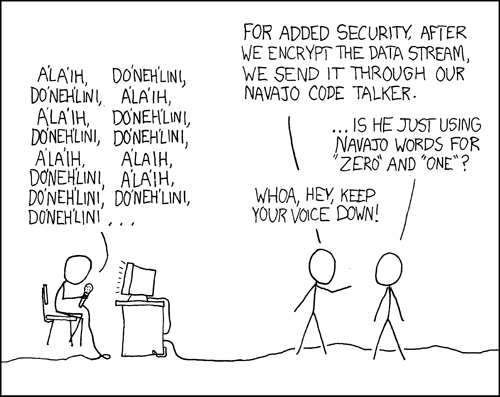
\includegraphics[width=\linewidth]{img/obscurity.png}
          \caption{XKCD 257}
        \end{figure}
    \end{column}
  \end{columns}
  \end{frame}
  \begin{frame}
    \slidetitle[L'absurdité de l'obscurité]
    \note{\ExecuteMetaData[008-evit_notes.tex]{Kerckhoffs}}
    \note{\ExecuteMetaData[008-evit_notes.tex]{Limites}}
    \begin{columns}
      \begin{column}{0.48\linewidth}
        \begin{block}{Principe de Kerckhoffs}<2->
          \centering
          \onslide<3->{
          ``Un système est considéré comme étant sécurisé de par sa conception et non parce que sa
          conception est inconnue de l'adversaire''
          }
        \end{block}
        \begin{block}{Les limites de l'obfuscation}<4->
          \begin{itemize}
          \item<5-> Débogage difficile
          \item<6-> Protection temporaire
          \item<7-> Potentiel perte de performances
          \item<8-> Qualité du code en baisse
          \item<9-> Appel à des librairies externes non obfuscables
          \end{itemize}
        \end{block}
      \end{column}
      \begin{column}{0.48\linewidth}
        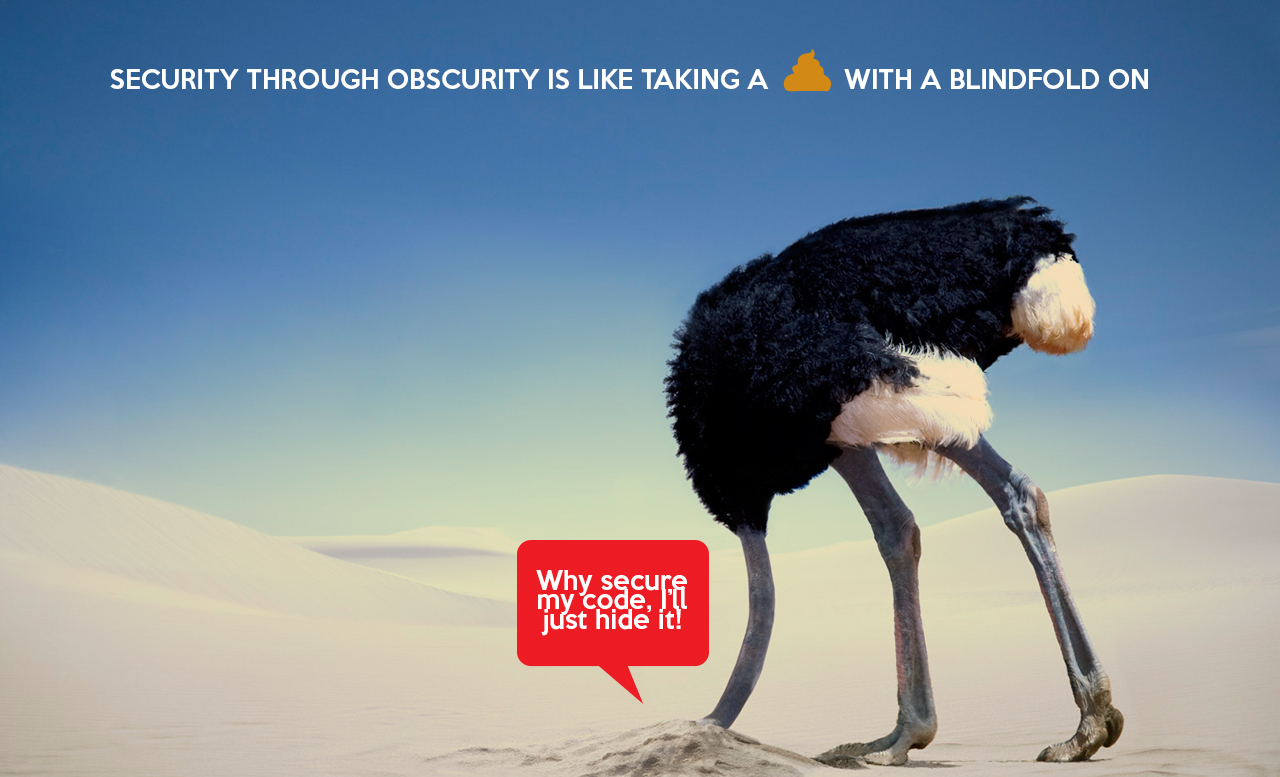
\includegraphics[width=\linewidth]{img/obscurity.jpg}
      \end{column}
    \end{columns}

    \end{frame}
\end{document}